\documentclass{article}
% translate with >> pdflatex -shell-escape <file>

% This file is an extract of the PGFPLOTS manual, copyright by Christian Feuersaenger.
% 
% Feel free to use it as long as you cite the pgfplots manual properly.
%
% See
%   http://pgfplots.sourceforge.net/pgfplots.pdf
% for the complete manual.
%
% Any required input files (for <plot table> or <plot file> or the table package) can be downloaded
% at
% http://www.ctan.org/tex-archive/graphics/pgf/contrib/pgfplots/doc/latex/
% and
% http://www.ctan.org/tex-archive/graphics/pgf/contrib/pgfplots/doc/latex/plotdata/

\usepackage{pgfplots}
\pgfplotsset{compat=newest}

\pagestyle{empty}

\usepgfplotslibrary{patchplots}

\begin{document}
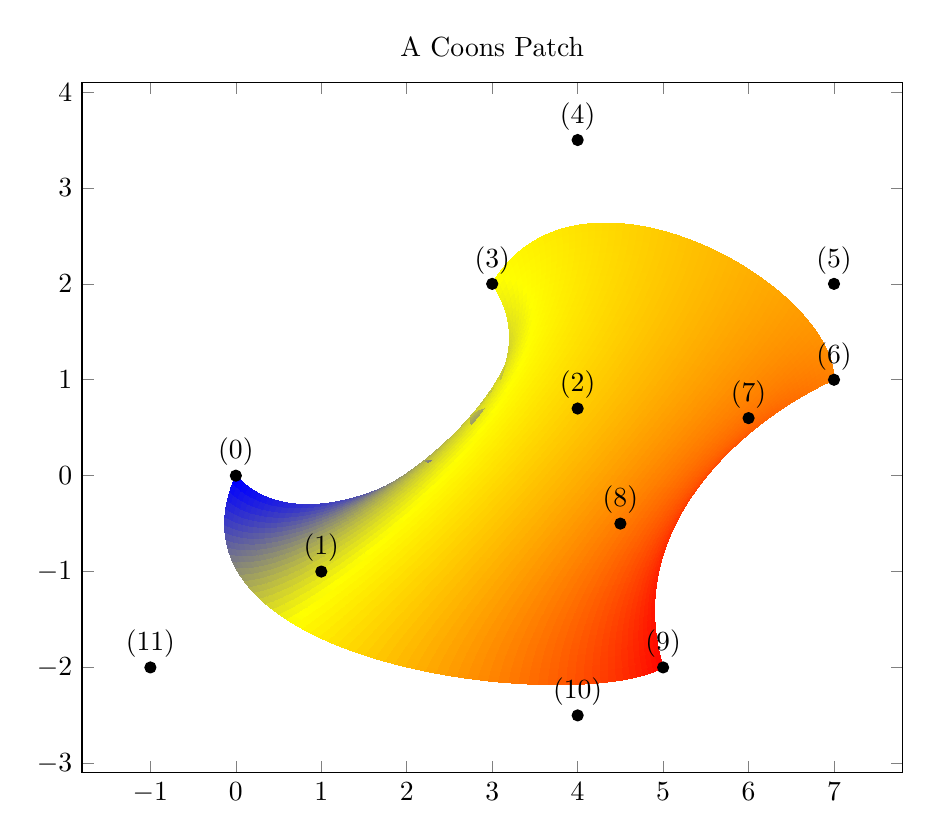
\begin{tikzpicture}
\begin{axis}[nodes near coords={(\coordindex)},
	width=12cm,
	title=A Coons Patch]
\addplot[mark=*,patch,patch type=coons,
	shader=interp,point meta=explicit] 
coordinates {
	(0,0)   [0] % first corner
	(1,-1)  [0] % Bezier control point between (0) and (3)
	(4,0.7) [0] % Bezier control point between (0) and (3)
	%
	(3,2)   [1] % second corner
	(4,3.5) [1] % Bezier control point between (3) and (6)
	(7,2)   [1] % Bezier control point between (3) and (6)
	%
	(7,1)      [2] % third corner
	(6,0.6)    [2] % Bezier control point between (6) and (9)
	(4.5,-0.5) [2] % Bezier control point between (6) and (9)
	%
	(5,-2)   [3] % fourth corner
	(4,-2.5) [3] % Bezier control point between (9) and (0)
	(-1,-2)  [3] % Bezier control point between (9) and (0)
};
\end{axis}
\end{tikzpicture}
\end{document}
